\section{Use-Case-Modell}

\textit{Alle identifizierten Use Cases werden in einer Übersicht in einem UML-Use-Case-Diagramm mit den dazugehörigen Akteuren dargestellt. Dabei soll das UML-Use-Case-Diagramm auch die Abgrenzung gegenüber externen Systemen darstellen (Systemkontext). \newline
Der oder die fachlich wichtigsten Use Cases müssen ausführlich fully dressed ausformuliert werden. Weitere wichtige Use Cases werden normal casual ausformuliert, während der Rest der Use Cases noch kurz brief beschrieben wird. Für das Standardszenario des fachlich wichtigsten und vollständig ausformulierten Use-Case wird ein System-Sequenzdiagramm (SSD) erstellt.
Für die wichtigsten Use-Cases werden UI-Sketches erstellt und allenfalls bei einem komplexeren UI die Navigationsmöglichkeiten (Dialogablauf) in einem Diagramm dargestellt. }

\subsection{Pdf-Generieren}

\begin{wrapfigure}{r}{6cm}
	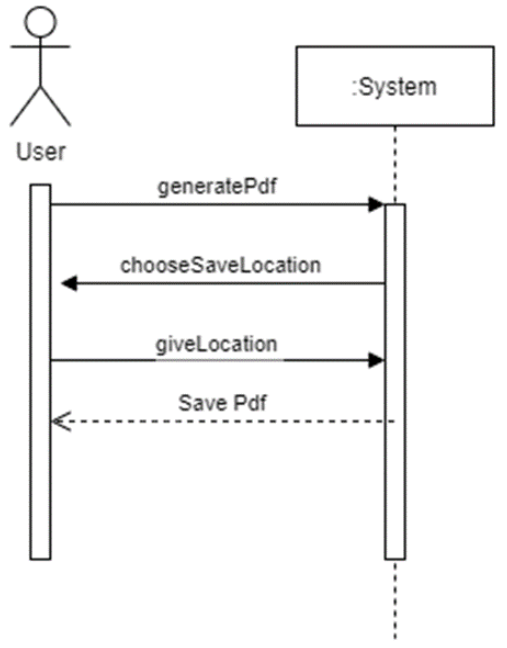
\includegraphics[width=6cm]{rec/UseCasePdfErstellen}
	\caption[SSD-Diagramm: Pdf-Generieren]{SSD-Diagramm: Pdf-Generieren}
	\label{fig:usecasepdferstellen}
\end{wrapfigure}
	
\textbf{Umfang:} aBrain Applikation \newline \newline
\textbf{Akteure:} Benutzende \newline \newline
\textbf{Stakeholders und Interessen:}  
\begin{itemize}
	\item Benutzer:innen (Primärakteur:in): Wollen unkompliziert eine Zusammenfassung mit den Journaleintragen, Erinnerungen etc als PDF haben.
	\item Therapeut:innen: Wollen die Daten der Benutzenden in möglichst einfacher und anschaulicher Form, um die Daten schneller zu verstehen und um die Therapie effizienter zu machen.
\end{itemize} 
\textbf{Vorbedingungen:} Benutzende haben ihr persönliches Profil erstellt und sind eingeloggt. \newline \newline
\textbf{Nachbedingungen:} Das Gerät braucht genügend Speicherplatz um die Datei abzulegen. Ausserdem muss ein gültiger Ordner / Speicherort ausgewählt werden. Ansonsten quittiert aBrain mit einer Fehlermeldung, dass der Speicherprozess fehlgeschlagen ist. Die Daten auf dem PDF müssen konsistent mit den Daten von aBrain sein. \newline \newline
\textbf{Standardablauf:} Die Benutzenden navigieren zum Statistikfenster und drücken auf den Knopf «PDF generieren.». Sobald die Datei generiert wurde, wird ein neues Fenster geöffnet und die Benutzenden werden gefragt, wo die Datei gespeichert werden soll. Anschliessend können die Benutzenden die Datei mit einer anderen Applikation anschauen oder verschicken. Therapeuten:innen können so unkompliziert den Zustand der Benutzenden untersuchen, falls diese ihnen ein solches PDF vor der Therapie zuschicken. \newline \newline
\textbf{Erweiterungen:} Es gibt die Möglichkeit vor dem Erstellen des PDFs gewisse Daten, beispielsweise die täglichen Moods, aus dem PDF auszuschliessen, dazu gibt es ein zusätzliches Menü mit Checkboxes. \newline \newline
\textbf{Spezielle Anforderungen:} Möglicherweise benötigt aBrain die Erlaubnis der Benutzenden, Dateien auf dem Gerät abzulegen. \newline \newline
\textbf{Häufigkeit des Auftretens:} Vor jeder Therapie. Die Anzahl Therapien pro Woche ist von Person zu Person unterschiedlich. 

\subsection{Nebenwirkung ins Journal eingeben }

\begin{wrapfigure}{r}{5cm}
	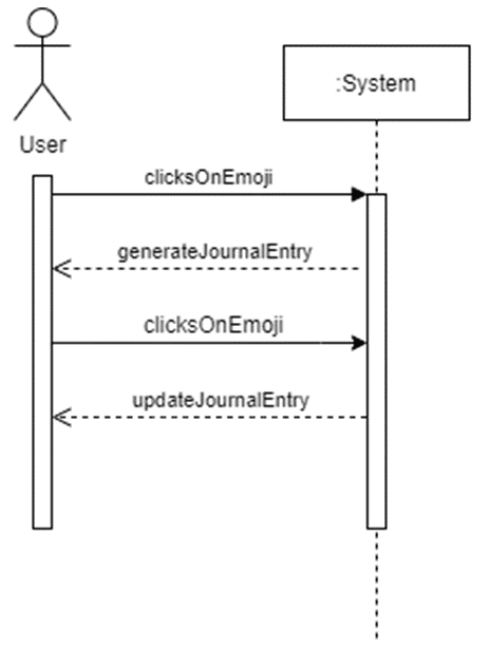
\includegraphics[width=6cm]{rec/UseCaseNebenwirkungJornal}
	\caption[SSD-Diagramm: Nebenwirkungen]{SSD-Diagramm: Nebenwirkungen}
	\label{fig:usecasenebenwirkungjornal}
\end{wrapfigure}


\textbf{Umfang:} aBrain Applikation \newline \newline
\textbf{Ebene:} Anwenderziel \newline \newline
\textbf{Primärakteur:} Benutzer:in \newline \newline
\textbf{Stakeholders und Interessen:}  
\begin{itemize}
	\item Benutzer:innen (Primärakteur): Wollen schnell und unkompliziert die Nebenwirkung eintragen. 
	\item Theraput:innen: Wollen eine genaue Beschreibung der Symptome und eine genaue Zeitangabe wann diese eingetroffen sind.
\end{itemize}
\textbf{Vorbedingungen:} Benutzende haben einen Account erstellt und sind eingeloggt. \newline \newline
\textbf{Nachbedingung:} Nebenwirkung ist im Journal gespeichert.  \newline \newline
\textbf{Standardablauf:} Die Benutzenden navigieren zum Journalfenster und klicken auf "neuer Journaleintrag". Ein neues Fenster öffnet sich und die Benutzenden suchen aus, was für ein Journaleintrag sie machen wollen. In diesem Fall klicken sie auf ''Mögliche Nebenwirkungen''. Nun schliesst sich das momentane Fenster und ein neues erscheint, sie können nun in einem Textfelfeld die genauen Symptome, sowie das vermutete Medikament notieren. Danach klicken sie auf ''Eintrag erstellen''. Ein Journaleintrag mit Zeitstempel und dem Titel ''Nebenwirkung'' wird erstellt.  \newline \newline
\textbf{Erweiterungen:} - 
\textbf{Spezielle Anforderungen:} -
\textbf{Liste der Technik:} -
\textbf{Häufigkeit des Auftretens:} Sehr selten \newline \newline

\subsection{Medikament eingeben}
\textbf{Umfang:} aBrain Applikation \newline \newline
\textbf{Akteure:} Benutzende \newline \newline
\textbf{Stakeholders und Interessen:}  
\begin{itemize}
	\item Benutzer:innen (Primärakteur): Wollen mit möglichst wenigen Klicks ein neues Medikament in ihrer Apotheke abspeichern.
\end{itemize}
\textbf{Vorbedingungen:} Benutzende haben einen Account erstellt und sind eingeloggt. \newline \newline
\textbf{Nachbedingungen:} Alle notwendigen Daten des Medikaments wurden eingegeben, ansonsten quittiert die App mit einer Fehlermeldung, wieso die Eingabe fehlgeschlagen ist \newline \newline
\textbf{Standardablauf:} Die Benutzenden navigieren zum Apothekenfenster und klicken auf den ''+'' Button (Medikament hinzufügen). Es öffnet sich ein neues Fenster als Pop-up, und die Benutzenden können nun die wichtigsten Daten des Medikaments eingeben: Wie viele Dosen in der Packung enthalten sind und wann das Medikament eingenommen werden soll. Zusätzlich gibt es ein Textfenster, wo man die bereits bekannten Nebenwirkungen notieren kann.  \newline \newline
\textbf{Erweiterungen:} Es gibt die Möglichkeit den Strichcode des Medikaments einzuscannen, um sich Klicks und Schreibarbeit zu ersparen. \newline \newline
\textbf{Spezielle Anforderungen:} Interne oder externe Datenbank mit den häufigsten Schweizer ADHS-Medikamenten. \newline \newline
\textbf{Liste der Technik:} - \newline \newline
\textbf{Häufigkeit des Auftretens:} Jedes Mal nachdem die Benutzenden ein neues Rezept erhalten. Das heisst dieser Use Case trifft selten ein. (Circa 1-5-mal pro Benutzer:in) \newline \newline

\subsection{Tägliche Stimmung eingeben }
\textbf{Umfang:} aBrain Applikation \newline \newline
\textbf{Akteure:} Benutzende \newline \newline
\textbf{Stakeholders und Interessen:}  
\begin{itemize}
	\item Benutzer:innen (Primärakteur): Wollen mit minimalem Aufwand täglich ihre Stimmung notieren
\end{itemize}
\textbf{Vorbedingungen:}  Benutzende haben einen Account erstellt und sind eingeloggt. \newline \newline
\textbf{Nachbedingungen:} \newline \newline
\textbf{Standardablauf:} Im Home Fenster gibt es vier Gesichter, traurig bis glücklich. Die Benutzenden klicken auf einen der vier Gesichtern. Ein Journaleintrag mit Zeitstempel und der ausgewählten Stimmung wird automatisch erstellt. Diese Auswahl lässt sich am selben Tag noch verändern, indem ein anderes Gesicht ausgewält wird. In diesem Fall wird auch der Journaleintrag korrekt nachgeführt. \newline \newline
\textbf{Erweiterungen:} Eine Erinnerung wird gesendet, falls die Stimmung am Abend noch nicht eingegeben wurde. \newline \newline
\textbf{Spezielle Anforderungen:} Die Möglichkeit, Push Benachrichtigungen / Erinnerungen an das Gerät zu senden. \newline \newline
\textbf{Liste der Technik:} - \newline \newline
\textbf{Häufigkeit des Auftretens:} Die Stimmung sollte jeden Tag eingegeben werden. \newline \newline

\subsection{ Wochenziel eingeben }
\textbf{Umfang:} aBrain Applikation \newline \newline
\textbf{Akteure:} Benutzende \newline \newline
\textbf{Stakeholders und Interessen:}  
\begin{itemize}
	\item Benutzer:innen (Primärakteur): Wollen mit minimalem Aufwand ein Wochenziel eingeben.
\end{itemize}
\textbf{Vorbedingungen:}  Benutzende haben einen Account erstellt und sind eingeloggt. \newline \newline
\textbf{Nachbedingungen:} \newline \newline
\textbf{Standardablauf:} Die Benutzenden navigieren zum Journal und tippen auf "Neues Wochenziel". Ein neues Fenster öffnet sich, und die Benutzer notieren im Textfeld ihr Ziel. Sobald die Benutzenden den Eintrag erstellt haben klicken sie auf "Eintrag erstellen". Ein neuer Journaleintrag wird mit Zeitstempel im Journal erstellt. Nach einer Woche bekommen die Benutzenden eine Push Nachricht. In der App öffnet sich nun ein neues Fenster mit zwei Buttons "Ziel erfüllt" oder "Ziel nicht erfüllt". Die Benutzenden klicken auf einen der beiden Buttons und schliessen somit das Wochenziel ab. \newline \newline
\textbf{Erweiterungen:} \newline \newline
\textbf{Spezielle Anforderungen:} Die Möglichkeit, Push Benachrichtigungen / Erinnerungen an das Gerät zu senden. \newline \newline
\textbf{Liste der Technik:} - \newline \newline
\textbf{Häufigkeit des Auftretens:} Etwa einmal pro Woche. \newline \newline